% =====================================================================
%  Chapitre 4 -- Apprentissage non supervisé (3 h)
%  Introduction au Machine Learning -- CNFSDP -- L3 S5 -- 2026-2027
%  Version niveau licence (12/10/2026)
%  Compilation : pdflatex chapitre4.tex (deux fois)
%  Figures : code/figures_chapitre4.py (données fictives : code/menages.py)
% =====================================================================
\documentclass[aspectratio=169,11pt]{beamer}
\usetheme{CNFSDP}
\usetikzlibrary{positioning,arrows.meta}
\usepackage{colortbl}

\chapitre{4}
\chapitrecourt{Ch.~4 \textendash{} Non supervisé}

\title{Chapitre 4 \textendash{} Apprentissage non supervisé}
\subtitle{Analyse en composantes principales, k-means, classification hiérarchique}
\author{Rois Céti DIMBAMBA}
\institute{Ingénieur statisticien économiste \textperiodcentered{} Actuaire \textperiodcentered{} \href{https://rdimbamba.shinyapps.io/roisceti_e-cv/}{\textcolor{cnfVert}{CV en ligne}}}
\date{22 octobre 2026}

\begin{document}

% ---------------------------------------------------------------------
\begin{frame}[plain,noframenumbering]
  \titlepage
\end{frame}

\begin{frame}{Plan et objectifs}
  \begin{columns}[T]
    \begin{column}{0.44\textwidth}
      \footnotesize\tableofcontents
    \end{column}
    \begin{column}{0.54\textwidth}
      \begin{objectifs}
        \footnotesize
        \begin{itemize}
          \item Résumer un tableau de nombreuses variables par l'ACP ; lire valeurs propres et cercle des corrélations.
          \item Comprendre comment se construit l'indice de richesse des enquêtes DHS.
          \item Regrouper des individus avec k-means et la classification hiérarchique.
          \item Choisir le nombre de groupes ; repérer des observations atypiques.
        \end{itemize}
      \end{objectifs}
      \vskip-1mm{\scriptsize\color{cnfGris}Prérequis : chapitre~0 (matrice de covariance, valeurs et vecteurs propres) et chapitre~1 (la moyenne est la meilleure constante).}
    \end{column}
  \end{columns}
\end{frame}

% =====================================================================
\section{Apprendre sans variable cible}

\begin{frame}{Le non supervisé}
  \begin{definition}[Apprentissage non supervisé]
    On observe seulement des variables $x_1,\dots,x_n\in\R^d$, sans variable cible $y$. On cherche une \emph{structure} dans les données : des directions qui résument l'information, ou des groupes d'individus qui se ressemblent.
  \end{definition}
  \begin{center}
    \small\renewcommand{\arraystretch}{1.3}
    \begin{tabular}{p{0.24\textwidth}p{0.3\textwidth}p{0.34\textwidth}}
      \toprule
      \textbf{Tâche} & \textbf{Méthodes} & \textbf{Exemple en statistique publique} \\
      \midrule
      Réduire la dimension & ACP & indice de richesse des enquêtes DHS \\
      Regrouper (classification non supervisée) & k-means, CAH & typologie des ménages \\
      Repérer l'atypique & forêt d'isolement & contrôle des questionnaires saisis \\
      \bottomrule
    \end{tabular}
  \end{center}
  {\small\color{cnfGris}Sans $y$, pas d'erreur de prédiction à mesurer : on juge un résultat par un critère (inertie) et par son interprétation.}
\end{frame}

% =====================================================================
\section{L'analyse en composantes principales}

\begin{frame}{Résumer $d$ variables par une seule}
  On part du tableau centré $X$ ($n$ lignes, $d$ colonnes, chaque colonne de moyenne nulle) et de sa matrice de covariance $S=\frac1nX\T X$ (chapitre~0).
  \begin{definition}[Composante, variance projetée]
    Pour une direction $u\in\R^d$ de norme $1$, la \emph{composante} $c=Xu$ donne à chaque individu le score $c_i=u_1x_{i1}+\dots+u_dx_{id}$. Sa variance vaut $\frac1n\norm{Xu}^2=u\T Su$.
  \end{definition}
  \begin{definition}[Axes principaux]
    Le \emph{premier axe} est la direction $u_1$, de norme $1$, qui rend la variance $u\T Su$ maximale. Le deuxième axe maximise la même variance parmi les directions orthogonales à $u_1$, et ainsi de suite.
  \end{definition}
  {\small\color{cnfGris}La contrainte $\norm u=1$ est indispensable : sans elle, on augmenterait la variance en allongeant $u$.}
\end{frame}

\begin{frame}{Le résultat central}
  \begin{theoreme}[Axes de l'ACP, admis]
    Les axes principaux sont les vecteurs propres de $S$, rangés selon leurs valeurs propres $\lambda_1\ge\lambda_2\ge\dots\ge\lambda_d\ge0$.
    La variance de la $k$-ième composante vaut $\lambda_k$.
  \end{theoreme}
  \begin{definition}[Inertie]
    L'\emph{inertie totale} est la somme des variances des $d$ variables. Elle vaut $\lambda_1+\dots+\lambda_d$ (admis). La part d'inertie \emph{expliquée} par l'axe $k$ est
    \[
      \frac{\lambda_k}{\lambda_1+\dots+\lambda_d}.
    \]
  \end{definition}
  \begin{aretenir}
    Faire une ACP, c'est diagonaliser la matrice de covariance : l'ordinateur le fait en une ligne (\texttt{np.linalg.eigh}, chapitre~0).
  \end{aretenir}
\end{frame}

\begin{frame}{Une ACP à la main}
  \small
  $4$ ménages, deux scores centrés : logement $x_1$ et équipement $x_2$ ; points $(-2,-1)$, $(-1,-2)$, $(1,2)$, $(2,1)$.
  \[
    S=\frac14X\T X=\frac14\begin{pmatrix}4+1+1+4&2+2+2+2\\2+2+2+2&1+4+4+1\end{pmatrix}=\begin{pmatrix}2{,}5&2\\2&2{,}5\end{pmatrix}.
  \]
  Toute direction de norme $1$ s'écrit $u=(\cos\theta,\sin\theta)$. Alors
  \[
    u\T Su=2{,}5\cos^2\theta+2{,}5\sin^2\theta+4\sin\theta\cos\theta=2{,}5+2\sin2\theta ,
  \]
  car $\cos^2\theta+\sin^2\theta=1$ et $2\sin\theta\cos\theta=\sin2\theta$.
  \begin{itemize}
    \item Maximum $2{,}5+2=4{,}5$ quand $\sin2\theta=1$, soit $\theta=45°$ : premier axe $u_1=\frac1{\sqrt2}(1,1)$.
    \item Minimum $2{,}5-2=0{,}5$ quand $\theta=135°$ : deuxième axe $u_2=\frac1{\sqrt2}(-1,1)$, orthogonal à $u_1$.
    \item Vérification : $Su_1=4{,}5\,u_1$ et $Su_2=0{,}5\,u_2$ : ce sont bien les vecteurs propres, et $\lambda_1=4{,}5$, $\lambda_2=0{,}5$.
  \end{itemize}
\end{frame}

\begin{frame}{L'ACP à la main en image}
  \centering
  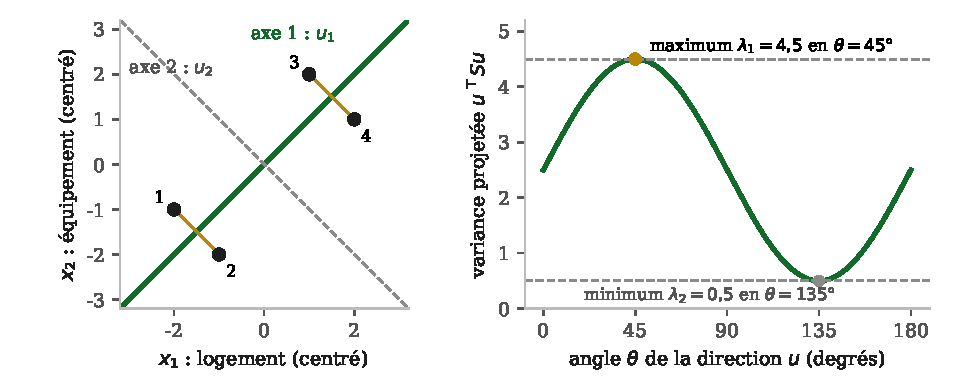
\includegraphics[width=0.74\textwidth]{acp_main.pdf}
  \vskip1mm
  \begin{minipage}{0.92\textwidth}
    \small
    À gauche : les $4$ ménages et leurs projections (en or) sur le premier axe. À droite : la variance projetée selon la direction choisie.
    \begin{itemize}
      \item Composante 1 : $c=\frac{x_1+x_2}{\sqrt2}\approx(-2{,}12;\,-2{,}12;\,2{,}12;\,2{,}12)$, de variance $4{,}5$.
      \item Part d'inertie expliquée : $4{,}5/(4{,}5+0{,}5)=90\,\%$ : un seul score résume presque tout.
    \end{itemize}
  \end{minipage}
\end{frame}

\begin{frame}{ACP normée}
  \begin{definition}[ACP normée]
    Quand les variables n'ont pas la même unité (revenu en FCFA, taille du ménage, années d'études), on les \emph{standardise} avant l'ACP : chaque colonne est centrée et divisée par son écart type.
    $S$ devient la matrice des corrélations, et l'inertie totale vaut $d$.
  \end{definition}
  \begin{itemize}\small
    \item Sans standardisation, la variable de plus grande variance (le revenu en FCFA) accaparerait le premier axe.
    \item Pour des variables binaires (le ménage possède ou non un bien), on standardise aussi : c'est la pratique de l'indice de richesse DHS.
  \end{itemize}
  \begin{remarque}[Combien d'axes garder ?]
    On regarde l'\emph{éboulis} des valeurs propres et l'on garde les premiers axes, avant le « coude ». En ACP normée, on garde souvent les axes de valeur propre supérieure à $1$ (règle de Kaiser), ou assez d'axes pour expliquer $70$ à $80\,\%$ de l'inertie.
  \end{remarque}
\end{frame}

\begin{frame}{Lire une ACP : éboulis et cercle des corrélations}
  \centering
  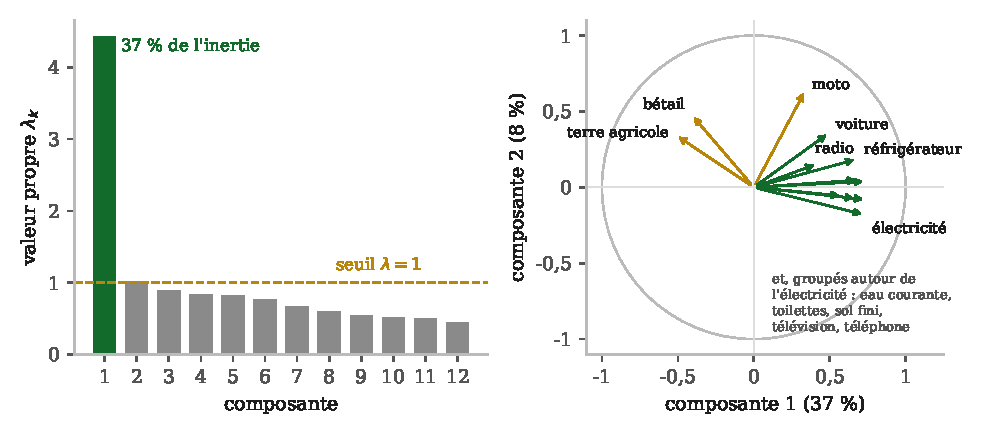
\includegraphics[width=0.76\textwidth]{eboulis_cercle.pdf}
  \vskip1mm
  \begin{minipage}{0.94\textwidth}
    \small
    $2\,000$ ménages fictifs, $12$ biens codés $0/1$ (électricité, eau courante\dots, bétail). Chaque flèche donne les corrélations d'un bien avec les deux composantes.
    L'axe 1 ($37\,\%$ de l'inertie) oppose les ménages sans équipement aux ménages équipés : c'est un axe de \emph{richesse}. L'axe 2 ($8\,\%$) distingue les biens ruraux (bétail, terre, moto).
  \end{minipage}
\end{frame}

\begin{frame}{Application : l'indice de richesse des enquêtes DHS}
  \begin{columns}[T]
    \begin{column}{0.55\textwidth}
      \small
      Les enquêtes démographiques et de santé ne mesurent pas le revenu. Elles construisent un \emph{indice de richesse} :
      \begin{enumerate}\setlength\itemsep{1pt}
        \item on relève les biens et les caractéristiques du logement de chaque ménage ;
        \item on fait une ACP normée sur ces variables ;
        \item le score de la \textbf{première composante} est l'indice de richesse ;
        \item on découpe l'indice en \textbf{quintiles} (les 20 \% les plus pauvres, etc.).
      \end{enumerate}
    \end{column}
    \begin{column}{0.42\textwidth}
      \begin{exemple}[Ménages fictifs]
        La richesse « cachée » qui a servi à simuler les biens est connue ici : sa corrélation avec la composante~1 vaut $0{,}895$.
        \vskip1mm
        Part des ménages avec réfrigérateur, par quintile :
        \begin{center}
          \begin{tabular}{ccccc}
            Q1 & Q2 & Q3 & Q4 & Q5 \\
            $1\,\%$ & $4\,\%$ & $17\,\%$ & $48\,\%$ & $91\,\%$
          \end{tabular}
        \end{center}
      \end{exemple}
    \end{column}
  \end{columns}
  \vskip1mm
  {\small\color{cnfGris}Projet : avec l'EDS Congo 2011-2012, vous pourrez reconstruire cet indice et le comparer à celui publié (variables \texttt{hv270}, \texttt{hv271}).}
\end{frame}

% =====================================================================
\section{Les k-means}

\begin{frame}{Regrouper : le critère d'inertie}
  \begin{definition}[Classification en $k$ groupes, inertie intra-classe]
    On cherche une partition des $n$ individus en $k$ groupes $G_1,\dots,G_k$. Chaque groupe a pour \emph{centre} la moyenne $c_j$ de ses individus. L'\emph{inertie intra-classe}
    \[
      W=\sum_{j=1}^k\;\sum_{i\in G_j}\norm{x_i-c_j}^2
    \]
    mesure la dispersion des individus autour du centre de leur groupe. On cherche la partition qui rend $W$ minimal.
  \end{definition}
  \begin{itemize}\small
    \item Des groupes compacts ont une petite inertie intra-classe.
    \item Essayer toutes les partitions est impossible : avec $n=100$ et $k=3$, il y en a plus de $10^{46}$.
    \item On utilise donc un algorithme qui améliore $W$ pas à pas.
  \end{itemize}
\end{frame}

\begin{frame}{L'algorithme de Lloyd (k-means)}
  \begin{definition}[k-means]
    On choisit $k$ centres de départ $c_1,\dots,c_k$, puis on répète jusqu'à ce que plus rien ne change :
    \begin{enumerate}\setlength\itemsep{1pt}
      \item \textbf{Affectation} : chaque individu rejoint le groupe du centre le plus proche ;
      \item \textbf{Mise à jour} : chaque centre devient la moyenne des individus de son groupe.
    \end{enumerate}
  \end{definition}
  \begin{proposition}
    Aucune des deux étapes ne fait augmenter l'inertie intra-classe $W$.
  \end{proposition}
  \begin{preuve}
    \textbf{Affectation} : chaque terme $\norm{x_i-c}^2$ est remplacé par la plus petite des distances aux centres, donc ne peut que baisser.
    \textbf{Mise à jour} : dans chaque groupe, la somme $\sum_i\norm{x_i-c}^2$ est minimale quand $c$ est la moyenne du groupe (la moyenne est la meilleure constante, chapitre~1, appliqué à chaque coordonnée).
  \end{preuve}
  {\small\color{cnfGris}Le nombre de partitions étant fini, l'algorithme s'arrête après un nombre fini d'itérations.}
\end{frame}

\begin{frame}{k-means à la main}
  \small
  Revenus mensuels de $6$ ménages (centaines de milliers de FCFA, fictifs) : $1,\ 2,\ 4,\ 6,\ 9,\ 12$. On prend $k=2$ et les centres de départ $1$ et $2$.
  \begin{center}
    \renewcommand{\arraystretch}{1.25}
    \begin{tabular}{cccc}
      \toprule
      itération & centres & groupes après affectation & $W$ \\
      \midrule
      0 & $1$ et $2$ & $\{1\}$ ; $\{2,4,6,9,12\}$ & $169$ \\
      1 & $1$ et $6{,}6$ & $\{1,2\}$ ; $\{4,6,9,12\}$ & $43{,}04$ \\
      2 & $1{,}5$ et $7{,}75$ & $\{1,2,4\}$ ; $\{6,9,12\}$ & $29{,}44$ \\
      3 & $2{,}33$ et $9$ & $\{1,2,4\}$ ; $\{6,9,12\}$ (inchangés) & $22{,}67$ \\
      \bottomrule
    \end{tabular}
  \end{center}
  {\footnotesize $W$ est calculé avec les centres de la ligne ; dernière ligne : $1{,}78+0{,}11+2{,}78+9+0+9\approx22{,}67$.}
  \vskip1mm
  \begin{remarque}[Un minimum seulement local]
    La partition $\{1,2,4,6\}$ ; $\{9,12\}$ a une inertie plus faible, $W=19{,}25$, et elle est aussi stable pour l'algorithme. Le résultat dépend du départ : on relance k-means avec plusieurs départs (\texttt{n\_init}) et l'on garde le meilleur $W$.
  \end{remarque}
\end{frame}

\begin{frame}{Lloyd en deux dimensions}
  \centering
  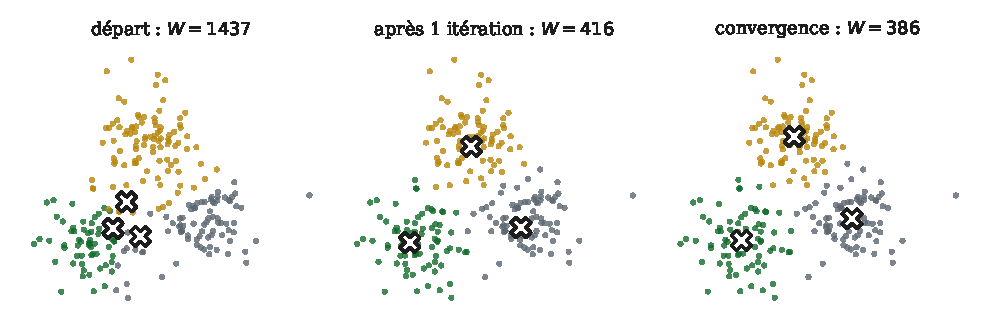
\includegraphics[width=0.9\textwidth]{lloyd.pdf}
  \vskip2mm
  \begin{minipage}{0.92\textwidth}
    \small
    $240$ points simulés en trois paquets ; les croix sont les centres. Partis de mauvais centres, regroupés en bas à gauche, ceux-ci migrent vers les trois paquets : $W$ passe de $1\,437$ à $386$.
    \vskip1mm
    {\color{cnfGris}En pratique, scikit-learn choisit des départs bien écartés (k-means++) et relance l'algorithme plusieurs fois. Comme pour le $k$-NN, on standardise les variables avant de calculer des distances.}
  \end{minipage}
\end{frame}

\begin{frame}{Choisir le nombre de groupes}
  \textbf{Coude.} $W(k)$ baisse toujours quand $k$ augmente ($W=0$ si chaque individu est seul) : on cherche le $k$ après lequel la baisse devient faible.
  \begin{definition}[Silhouette]
    Pour l'individu $i$, soit $a$ sa distance moyenne aux membres de son groupe et $b$ sa distance moyenne aux membres du groupe voisin le plus proche :
    \[
      s(i)=\frac{b-a}{\max(a,b)}\in[-1,1].
    \]
    Proche de $1$ : bien classé ; négatif : plus proche de l'autre groupe. On choisit le $k$ qui maximise la silhouette moyenne.
  \end{definition}
  \begin{exemple}
    Partition $\{1,2,4,6\}$ ; $\{9,12\}$, ménage de revenu $4$ : $a=\frac{3+2+2}3\approx2{,}33$, $b=\frac{5+8}2=6{,}5$, d'où $s=\frac{6{,}5-2{,}33}{6{,}5}\approx0{,}64$ : bien classé.
  \end{exemple}
\end{frame}

\begin{frame}{Coude et silhouette en pratique}
  \centering
  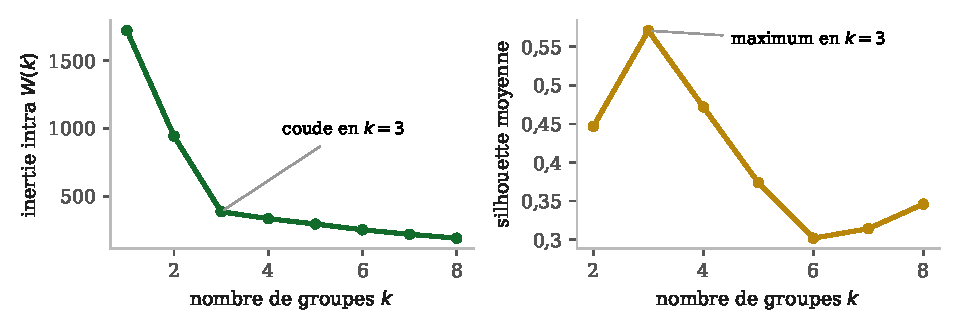
\includegraphics[width=0.86\textwidth]{coude.pdf}
  \vskip2mm
  \begin{minipage}{0.9\textwidth}
    \small
    Les $240$ points en trois paquets de la diapositive précédente : $W(k)$ chute jusqu'à $k=3$ puis baisse lentement, et la silhouette est maximale en $k=3$.
    Sur des données réelles, les critères sont rarement aussi nets : on les croise avec l'interprétation des groupes.
  \end{minipage}
\end{frame}

% =====================================================================
\section{La classification hiérarchique}

\begin{frame}{Classification ascendante hiérarchique (CAH)}
  \begin{definition}[CAH, critère de Ward]
    On part de $n$ groupes d'un seul individu. À chaque étape, on fusionne les deux groupes $A$ et $B$ dont la fusion fait le moins augmenter l'inertie intra-classe. Avec le critère de Ward, cette hausse vaut (admis)
    \[
      \Delta(A,B)=\frac{n_An_B}{n_A+n_B}\,\norm{c_A-c_B}^2 ,
    \]
    où $n_A$, $n_B$ sont les effectifs et $c_A$, $c_B$ les centres. On s'arrête quand il ne reste qu'un groupe.
  \end{definition}
  \small
  \begin{itemize}
    \item L'historique des fusions se dessine en \emph{dendrogramme} : la hauteur d'une fusion est son coût $\Delta$.
    \item On coupe l'arbre là où les fusions deviennent chères : on obtient le nombre de groupes.
    \item Pas de départ au hasard : le résultat est toujours le même.
  \end{itemize}
\end{frame}

\begin{frame}{CAH à la main sur les six ménages}
  \begin{columns}[T]
    \begin{column}{0.56\textwidth}
      \small
      \renewcommand{\arraystretch}{1.25}\setlength\tabcolsep{4pt}
      \begin{tabular}{clc}
        \toprule
        étape & fusion & hausse $\Delta$ \\
        \midrule
        1 & $\{1\}+\{2\}$ & $\frac{1\times1}{2}\times1^2=0{,}5$ \\
        2 & $\{4\}+\{6\}$ & $\frac12\times2^2=2$ \\
        3 & $\{9\}+\{12\}$ & $\frac12\times3^2=4{,}5$ \\
        4 & $\{1,2\}+\{4,6\}$ & $\frac{2\times2}{4}\times3{,}5^2=12{,}25$ \\
        5 & $\{1,2,4,6\}+\{9,12\}$ & $\frac{4\times2}{6}\times7{,}25^2\approx70{,}08$ \\
        \bottomrule
      \end{tabular}
      \vskip2mm
      En coupant avant la dernière fusion, très chère, on obtient $2$ groupes : $\{1,2,4,6\}$ et $\{9,12\}$, d'inertie intra $0{,}5+2+12{,}25+4{,}5=19{,}25$.
    \end{column}
    \begin{column}{0.42\textwidth}
      \centering
      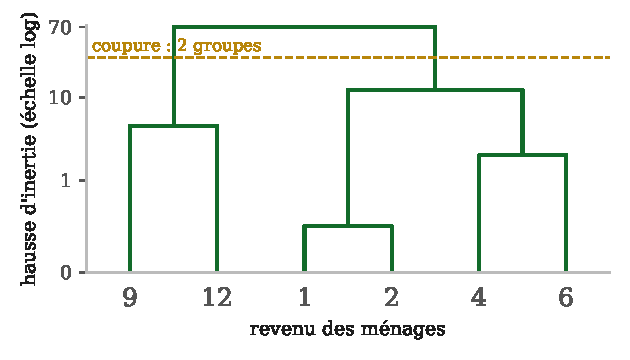
\includegraphics[width=\textwidth]{dendrogramme.pdf}
      {\scriptsize\color{cnfGris}La CAH retrouve ici la meilleure partition, que k-means parti de $1$ et $2$ avait manquée.}
    \end{column}
  \end{columns}
\end{frame}

\begin{frame}{Inertie totale, intra et inter}
  \begin{proposition}[Décomposition de Huygens, admise]
    Pour toute partition, l'inertie totale $T=\sum_i\norm{x_i-\bar x}^2$ se décompose en
    \[
      T=\underbrace{\sum_j\sum_{i\in G_j}\norm{x_i-c_j}^2}_{W\text{ : intra-classe}}+\underbrace{\sum_jn_j\norm{c_j-\bar x}^2}_{B\text{ : inter-classe}} .
    \]
  \end{proposition}
  \small
  \textbf{Vérification} : moyenne $\bar x=\frac{34}6\approx5{,}67$ et $T\approx89{,}33$.
  Pour $\{1,2,4,6\}$ ; $\{9,12\}$ : $W=19{,}25$ et $B=4\times(3{,}25-5{,}67)^2+2\times(10{,}5-5{,}67)^2\approx70{,}08$, d'où $W+B=89{,}33$.
  \begin{remarque}[Lecture]
    $T$ ne dépend pas de la partition : minimiser l'inertie intra revient à maximiser l'inertie inter, c'est-à-dire à séparer les groupes. La part $B/T$ (ici $78\,\%$) mesure la qualité d'une partition, comme un $R^2$.
  \end{remarque}
\end{frame}

\begin{frame}{k-means ou CAH ?}
  \small
  \renewcommand{\arraystretch}{1.2}
  \begin{tabular}{p{0.22\textwidth}p{0.33\textwidth}p{0.33\textwidth}}
    \toprule
    & \textbf{k-means} & \textbf{CAH (Ward)} \\
    \midrule
    Nombre de groupes & fixé à l'avance & choisi en coupant le dendrogramme \\
    Résultat & dépend du départ (minimum local) & toujours le même \\
    Grands effectifs & rapide, même pour $n=100\,000$ & lent : compare tous les groupes deux à deux \\
    Forme des groupes & groupes compacts, de tailles voisines & idem avec Ward \\
    \bottomrule
  \end{tabular}
  \vskip2mm
  \begin{aretenir}
    Stratégie classique : ACP pour résumer les variables, puis CAH ou k-means sur les premières composantes, puis description de chaque groupe par les moyennes des variables d'origine.
  \end{aretenir}
\end{frame}

\begin{frame}{Une typologie de ménages}
  \small
  k-means à $3$ groupes sur les deux premières composantes des $2\,000$ ménages fictifs. Part des ménages possédant le bien :
  \begin{center}
    \renewcommand{\arraystretch}{1.25}
    \begin{tabular}{lcccc}
      \toprule
      groupe & effectif & électricité & voiture & bétail \\
      \midrule
      ménages ruraux peu équipés & $870$ & $21\,\%$ & $1\,\%$ & $55\,\%$ \\
      ménages équipés sans véhicule & $715$ & $90\,\%$ & $3\,\%$ & $14\,\%$ \\
      ménages aisés & $415$ & $96\,\%$ & $55\,\%$ & $23\,\%$ \\
      \bottomrule
    \end{tabular}
  \end{center}
  \begin{itemize}
    \item On nomme les groupes \emph{après coup}, en lisant leurs moyennes : l'algorithme ne connaît que des numéros.
    \item La CAH de Ward donne le même groupe pour $91\,\%$ des ménages.
    \item La silhouette préférerait $2$ groupes ; $3$ groupes restent lisibles. Le choix final mêle critères et interprétation.
  \end{itemize}
\end{frame}

% =====================================================================
\section{Repérer l'atypique}

\begin{frame}{La forêt d'isolement}
  \begin{columns}[T]
    \begin{column}{0.62\textwidth}
      \begin{definition}[Forêt d'isolement]
        On construit de nombreux arbres \emph{au hasard} (variable et seuil tirés au sort à chaque nœud) jusqu'à isoler chaque individu.
        Un individu atypique est isolé en \emph{peu} de coupures : son score d'anomalie est élevé si sa profondeur moyenne d'isolement est faible.
      \end{definition}
      \footnotesize
      \begin{itemize}\setlength\itemsep{0pt}
        \item Méthode d'ensemble (chapitre~3), sans variable cible.
        \item Usages : contrôle de saisie des questionnaires, fraudes, valeurs aberrantes.
        \item Ménages fictifs : les $1\,\%$ les plus atypiques mêlent biens « urbains » (réfrigérateur, voiture) et « ruraux » (bétail, moto).
        \item Atypique ne veut pas dire faux : on vérifie avant d'exclure.
      \end{itemize}
    \end{column}
    \begin{column}{0.36\textwidth}
      \centering
      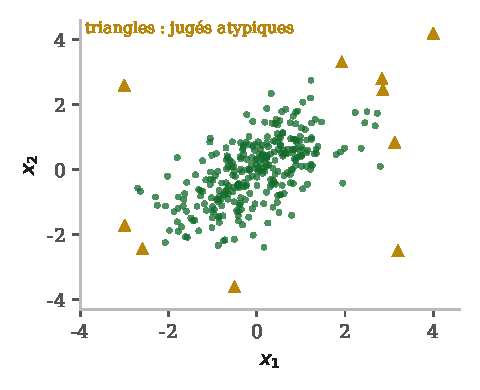
\includegraphics[width=\textwidth]{isolement.pdf}
      {\scriptsize\color{cnfGris}$300$ points simulés et $5$ points ajoutés à l'écart.}
    \end{column}
  \end{columns}

\end{frame}

% =====================================================================
\section{En Python}

\begin{frame}[fragile]{ACP et indice de richesse}
\begin{python}[basicstyle=\ttfamily\scriptsize]
import numpy as np, pandas as pd
from sklearn.preprocessing import StandardScaler
from sklearn.decomposition import PCA

biens, richesse, urbain = simuler_menages()      # TP4 : 2 000 ménages fictifs, 12 biens (0/1)
Z = StandardScaler().fit_transform(biens)        # ACP normée
acp = PCA().fit(Z)
print(acp.explained_variance_[:3].round(2))      # valeurs propres : [4.43 1.02 0.88]
print(acp.explained_variance_ratio_[:2].round(3))  # parts d'inertie : [0.369 0.085]
indice = acp.transform(Z)[:, 0]                  # indice de richesse = composante 1
if np.corrcoef(indice, biens["electricite"])[0, 1] < 0:
    indice = -indice                             # orienter : plus riche = plus grand
print(round(np.corrcoef(indice, richesse)[0, 1], 3))   # lien avec la richesse cachée : 0.895
quintile = pd.qcut(indice, 5, labels=False) + 1
print(biens.groupby(quintile)["refrigerateur"].mean().round(2).values)
# [0.01 0.04 0.17 0.48 0.91]
\end{python}
\vskip-1mm
{\small\color{cnfGris}Le signe d'une composante est arbitraire : on l'oriente pour que l'indice croisse avec la richesse.}
\end{frame}

\begin{frame}[fragile]{k-means, CAH et forêt d'isolement}
\begin{python}[basicstyle=\ttfamily\scriptsize]
from sklearn.cluster import KMeans, AgglomerativeClustering
from sklearn.metrics import silhouette_score
from sklearn.ensemble import IsolationForest

C = acp.transform(Z)[:, :2]                      # deux premières composantes
for k in [2, 3, 4, 5]:
    km = KMeans(n_clusters=k, n_init=10, random_state=0).fit(C)
    print(k, round(km.inertia_), round(silhouette_score(C, km.labels_), 3))
# 2 4129 0.516 | 3 2771 0.454 | 4 2075 0.398 | 5 1634 0.426
km = KMeans(n_clusters=3, n_init=10, random_state=0).fit(C)
cah = AgglomerativeClustering(n_clusters=3, linkage="ward").fit(C)
print(pd.crosstab(km.labels_, cah.labels_))      # 91 % des ménages dans le même groupe
print(biens.groupby(km.labels_)[["electricite", "voiture", "betail"]].mean().round(2))
iso = IsolationForest(contamination=0.01, random_state=0).fit(Z)
print(biens[iso.predict(Z) == -1].mean().round(2))     # profil des 20 ménages atypiques
\end{python}
\vskip-1mm
{\small\color{cnfGris}\texttt{contamination} fixe la part d'individus déclarés atypiques ($1\,\%$ ici).}
\end{frame}

% =====================================================================
\section{TP en salle}

\begin{frame}{TP4 \textendash{} ACP, k-means, CAH}
  \footnotesize
  \begin{tp}{TP4 \textendash{} à faire en salle}{45 min \textperiodcentered{} \texttt{notebooks/TP4.ipynb} (Colab)}
    \begin{enumerate}\setlength\itemsep{0pt}
      \item \textbf{ACP à la main} : pour les $4$ ménages du cours, calculer $S$, ses valeurs et vecteurs propres, et tracer $u\T Su$ en fonction de l'angle.
      \item \textbf{Indice de richesse} : ACP normée des $2\,000$ ménages fictifs ; éboulis, corrélations avec les axes, indice et quintiles ; comparer à la richesse cachée.
      \item \textbf{Lloyd en NumPy} : programmer k-means sur les $6$ revenus ; partir des centres $1$ et $2$, puis $3$ et $11$ ; comparer les inerties.
      \item \textbf{Nombre de groupes} : coude et silhouette pour $k=2,\dots,8$ sur les ménages ; décrire les groupes retenus.
      \item \textbf{CAH} : dendrogramme des $6$ revenus avec \texttt{scipy} ; retrouver les coûts de fusion du cours ; vérifier $T=W+B$.
      \item \textbf{Forêt d'isolement} : repérer les $1\,\%$ de ménages les plus atypiques et décrire leur profil.
    \end{enumerate}
  \end{tp}
\end{frame}

\begin{frame}{Résumé}
  \begin{itemize}\small
    \item Non supervisé : pas de $y$ ; on cherche des directions (ACP) ou des groupes (k-means, CAH).
    \item ACP : axes = vecteurs propres de la covariance, variances = valeurs propres ; standardiser si les unités diffèrent ; lire l'éboulis et les corrélations avec les axes.
    \item L'indice de richesse DHS est la première composante d'une ACP sur les biens des ménages.
    \item k-means : affectation au centre le plus proche, puis centres = moyennes ; l'inertie intra ne remonte jamais, mais le minimum peut n'être que local.
    \item CAH de Ward : fusions successives au moindre coût d'inertie ; dendrogramme ; résultat déterministe.
    \item $T=W+B$ : bien regrouper, c'est séparer les groupes. On choisit $k$ par le coude, la silhouette et l'interprétation.
    \item Forêt d'isolement : les individus isolés en peu de coupures sont atypiques.
  \end{itemize}
\end{frame}

\end{document}
